\section{Method}
\label{sec:method}

The review aspect extraction problem aims to extract or infer $K$ noun 
words from user review texts,
each word should represent a distinct aspect or feature of a type of product or service. 
Here $K$ is an constant parameter for the problem. 
In unsupervised models for aspect extraction, 
the set of reviews and the number of aspects are the only inputs.
Note that in this definition we don't use cross-domain information, 
that is, for one product type we only use the reviews of that domain.
This allows us to apply the model to any domain with ease.

\begin{figure}[th]
\centering
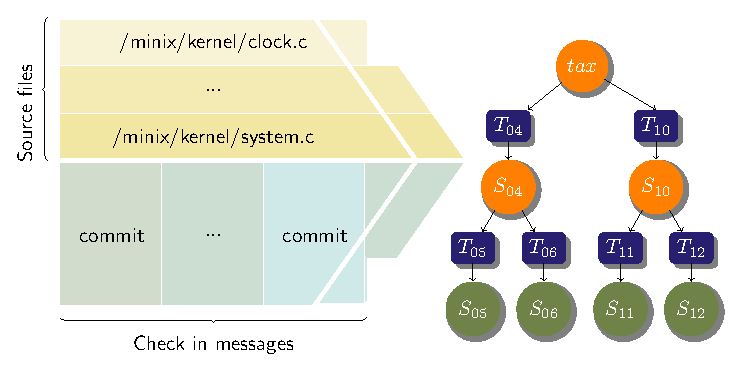
\includegraphics[width=0.9\columnwidth]{figures/framework}
\caption{Our framework.}
\label{fig:framework}
\end{figure}

The framework of our method is shown in \figref{fig:framework}, 
it consists of 5 steps:

\begin{itemize}
    \item \textbf{Sentence Clustering}

        We convert each sentence in the reviews into a vector representation 
        and cluster them in to $N$ clusters of semantically similar sentences.

    \item \textbf{Noise Isolation}

        %As aspects appear as topics in the reviews, 
        %we use a topic model to infer the potential aspects.
        To isolate the noises that exist in the sentence cluster,
	for each sentence cluster we further generate $M$ 
	topics, resulting in $N\times M$ different word distributions in total.

    \item \textbf{Aspect Inference}
        
        We treat each word distribution as a vector and cluster the topics 
	into $C$ clusters which are the potential aspects. 
	Here $C$ is purposely set to be larger than $K$. The extra
	$C-K$ clusters models the redundant aspects.
        Each cluster contains $N\times M / C$ word distributions, or vectors.
        We take the mean of these vectors to form $C$ aspect clusters,
        each being a set of words and their corresponding weights.

    \item \textbf{Cluster Ranking}

        We define a score for the quality of each aspect cluster,
        and the clusters are ranked by this score.

    \item \textbf{Word Ranking}

        We use WordNet to calculate the semantic distances between the words 
	in each cluster and adjust the ranking based on the 
	both the distances and the weights of the words. The top words in each
	cluster are candidates of the aspect words.
\end{itemize}

In the following we will explain the motivation and the details of each of
the five steps. 

\subsection{Sentence Clustering}

One important feature of user reviews is that many topics are 
compressed into a short paragraph, where each topic corresponds to 
a potential aspect of the product. 
A typical hotel review extracted from \figref{fig:tripadvisor} 
is shown as follows:

\begin{quote}
Pool is small and only 4 ft but refreshing. Hot tub also there. Staff were super friendly each day. Room was nothing special but clean and comfy. Lots of restaurants and bars nearby. Breakfast was great and despite being a busy weekend there was always a big selection available.
\end{quote}

In user reviews, topics can shift very quickly.
Sentences that are close to each other may refer to 
completely different aspects about the product. Also,
sentences about the same aspect may not appear in the review consecutively. 
The existence of such fine-grained semantic shifts in user reviews 
makes it difficult to apply the the bag-of-word abstraction 
of normal topic model on reviews.
Therefore we propose to work on the sentence level instead 
of the document level, and it would be helpful if we can divide the 
reviews into topic-oriented segments.

Driven by this observation, in our method the first step is 
sentence clustering.  For this purpose, we represent each 
sentence in a high-dimensional vector space.
Instead of using simplistic methods like bag-of-word vector, 
we leverage a recent development of neural network in natural 
language processing, the distributed representation.
In a distributed representation, words and sentences are 
converted into real-valued vectors.
The distance of the vectors in the vector space will capture the 
semantic similarity of the words or sentences.
In this work we attempt two models, recurrent neural network (RNN) and paragraph vector (PV) \cite{le2014distributed}.

\paragraph{Recurrent Neural Network}
To use RNN for obtaining sentence vectors, 
we train a neural language model on the review sentences. 
After the perplexity converges, we use the trained network to 
process each sentence of the dataset and take the last hidden vector as 
the vector representation of the sentence. In our method we use a 
variation of RNN, long-short term memory (LSTM)~\cite{hochreiter1997long} 
which is reported to have better performance at 
modeling long sentences \cite{jozefowicz2015empirical}.

\paragraph{Paragraph Vector}
PV is a simple but powerful extension to Word2vec \cite{mikolov2013distributed} with two components, 
distributed memory (PV-DM) and distributed bag-of-word (PV-DBOW). 
The first one is similar to skip-gram in Word2vec and 
the second is similar to CBOW \cite{mikolov2013distributed}.
An important advantage of paragraph vector models is that they require 
no labeled data. Also, it doesn't require human experts to assign weights 
for words in a paragraph based on linguistic knowledge. 
The learned vector representations inherit an important property of Word2vec, 
that is the semantics similarity. Also the final paragraph vector captures the 
word order information with the part learned from PV-DBOW with the n-gram model.
In practice, an advantage of paragraph vector over RNNs is that it can 
leverage trained word vectors. The word vectors can be trained on 
a much larger corpus so they capture the semantics relationships more 
accurately.  Consequently, the paragraph vectors can be trained on 
a relatively small dataset. 
The performance of paragraph vectors can also be boosted by using pre-trained 
word vectors that are trained on a larger dataset \cite{mikolov2013linguistic}. 
%However, previous research show that it is more suitable 
%to train the word vectors simultaneously for RNNs, 
%so RNNs cannot leverage the word vectors learned from a larger dataset. 
Also, the paragraph vector models are simple and 
don't require the storage of a lot of information. In contrast, for RNN we 
need to store every state during the forward pass for back-propagation, 
which is very memory consuming.

\paragraph{Clustering Sentence Vectors}
We run a k-means clustering on the sentence vectors and generate 
$N$ sentence clusters. We then collect the sentences from the same review 
that are clustered together to form smaller pieces of reviews. 
Each review document is divided into several shorter documents, each belonging
to one of the $N$ clusters. As a result, we obtain $N$ clusters of shorter documents. 

\subsection{Noise Isolation}
The first step, sentence clustering, we might include noise and the sentences 
within a cluster might not all be about the same aspect. 
The reason is due to the common occurrences of sentences such as the following
in the reviews (taken from TripAdvisor):

\begin{quote}
The room was clean, the staff were friendly, and I would say the price is very reasonable given the proximity to business and leisure destinations around downtown.
\end{quote}

\begin{quote}
There is a restaurant just 5 min walk away with nice italian food, pizza was great.
\end{quote}

In the first sentence multiple aspects are mentioned; in the second sentence, the only aspect is location however lexically it seems to be talking about food.
With these complicated structures within, 
it is difficult for RNN or PV to correctly determine the aspects 
in these sentences. The result is overlaps between clusters about 
different aspects and noises within each cluster.
To isolate the noises and resolve such overlap, 
We apply LDA \cite{blei2003latent} topic modeling within each sentence cluster, 
treating each review piece as a document, and generating $M$ smaller topics. 
This will give us in total $N\times M$ topics, or, word distributions. 
\tabref{table:overlap} shows an example of topics inferred from three
sentence clusters from hotel reviews and illustrates the overlap problem.
In this example, five topics were extracted from each sentence cluster, 
and each row is one topic. It can be seen that the aspects for the 
three clusters should be {\em room}, {\em location} and {\em price} 
respectively.
However, topics shown in boldface font obviously belong to 
other clusters.  Especially, the last topic of the third cluster 
appears to be an overlap of more than two clusters.
The noise isolation step effectively separates the noise topics from other
topics semantically corehent within a sentence cluster.

\begin{table}[th]
\centering
\caption{Topics extracted from three sentence clusters of hotel review.}
\label{table:overlap}
\begin{tabular}{|c|l|}
\hline
& room bed bedroom size floor \\
Sentence
& bedroom room wall size decor \\
cluster 1
& room bathroom shower water towel \\
& room suite size view floor \\
& room shower area kitchen bed \\\hline

& station minute tube location bus \\
Sentence
& location price night place rate\\
cluster 2
& location square station street subway\\
& distance bus subway downtown shopping\\
& \textbf{restaurant} \textbf{city} \textbf{food} \textbf{buffet} \textbf{place} \\\hline

& price rate service money star\\
Sentence
& \textbf{location} \textbf{city} \textbf{star} \textbf{time} \textbf{rate} \\
cluster 3
& price service night money city\\
& price location place night city\\
& \textbf{location} \textbf{service} \textbf{food} \textbf{price} \textbf{restaurant} \\\hline
\end{tabular}
\end{table}


\subsection{Aspect Inference}
\label{sec:topic_clustering}

The overlapping topics can be distinguished from other topics from the 
same cluster by comparing their word distributions, 
and in this step we resolve this overlapping and infer the candidate
aspects.

We treat each topic as a vector, where an entry is the frequency of a word. 
These vectors have dimensionality equal the size of the vocabulary, which is too large for clustering, 
so we perform dimensionality reduction these vectors.
Specifically, we use PCA to reduce the topics vectors to 100-dimensional. 
By doing this, we select the 100 most words that best distinguish different topics.

Then we perform a k-means on the $N\times M$ topics vectors to 
generate $C$ clusters, each containing $(N\times M)/C$ topics.
Because of the existence of noisy topics as the last topic shown 
in \tabref{table:overlap}, we need to set $C$ slightly larger than 
the desired number of product aspects $K$,
so that the noisy topics can be clusters together and later discarded. 
In an experiment we will evaluate the influence of this redundant clusters on 
the quality of the final aspects.

\begin{table}[th]
\caption{Aspect clusters extracted from hotel reviews.
Each row shows the candidate words of an aspect, sorted by the weight of each word.}
\label{table:step3}
\centering
\begin{tabular}{|l|} \hline
breakfast, meal, food, tasty, dinner, morning, coffee, tea \\\hline
room, night, time, bed, day, bathroom, staff, area, place \\\hline
staff, desk, service, friendly, reception, concierge, helpful \\\hline
close, city, location, place, central, station, bus, street\\\hline
bed, shower, spacious, room, size, bathroom, bedroom, floor \\\hline
price, room, check, night, money, city, location, star, service \\\hline
location, price, room, night, place, rate, money, time, city  \\\hline
\end{tabular}
\end{table}

Finally, for each cluster we take the mean of the $(N\times M)/C$ topics and normalize it
for the word distribution of that cluster.
We call them {\em aspect clusters}.
Some example aspect clusters extracted from hotel reviews are 
shown in \tabref{table:step3}.

\subsection{Cluster Ranking}

In the previous step, we have formed $C$ aspect clusters, with the possibilities
of a few noise clusters.  In this step,
we discard the $C-K$ noisy clusters. 
To identify the noisy clusters, we design a {\em distinctiveness score} 
to measure the quality of the clusters. 

The distinctiveness of a cluster measures how different it is 
from other clusters. Intuitively, if a cluster is 
similar to other clusters, it is likely to be the result of overlaps,
thus it is said to have a lower quality. 
For the $i$th cluster $C_i$ ($i\in [1, C]$), 
the distinctiveness score $S(i)$ is defined by:

\begin{align}
S(i) &= \sum_{w\in C_i} S_i(w) \nonumber\\ 
     &= \sum_{w\in C_i} \log\left(\frac{f_i(w)}{\sum_{j\neq i} f_j(w)}\right)\nonumber \\
     &= \sum_{w\in C_i}\left[\log f_i(w) - \log\sum_{j\neq c} f_j(a)\right]
\end{align}

Subsequently, the clusters are ranked in the decending order of 
this score and the last $C-K$ clusters are discarded.
The result is shown in \tabref{table:clustersranked}, the discarded cluster are greyed-out.

\begin{table}[t]
\caption{Aspect clusters ranked by distinctiveness score.
Potential aspect words are boldfaced.}
\label{table:clustersranked}
\centering
\begin{tabular}{|l|} \hline
\textbf{staff}, desk, \textbf{service}, friendly, reception, concierge, helpful \\\hline
breakfast, meal, \textbf{food}, tasty, dinner, morning, coffee, tea \\\hline
\textbf{price}, room, check, night, money, city, location, star, service \\\hline
bed, shower, spacious, \textbf{room}, size, bathroom, bedroom, floor \\\hline
close, city, \textbf{location}, place, central, station, bus, street \\\hline
\textcolor{mygray}{room, night, time, bed, day, bathroom, staff, area, place} \\\hline
\textcolor{mygray}{location, price, room, night, place, rate, money, time, city} \\\hline
\end{tabular}
\end{table}

\subsection{Word Ranking}
\label{sec:word_ranking}


In \tabref{table:clustersranked},
we manually selected and boldfaced the the most representative words for
each cluster, shown in boldface.  
Each of these words can act as a summary of the 
other words in the same cluster, and can serve as the aspect words.
However, it can be seen that not all of them have the highest frequency 
in their clusters.  In order to 
automatically select the best aspect words,
in this ranking step we adjust the order of the word in cluster 
by considering both the weights and the semantics of the words.

The weights of the words are given in the aspect inference step.
We keep only nouns from this step since the appropriate aspects 
should be nouns. The most prominent and representative word in each cluster
is assumed to be the closest to the centroid of the word cluster.
To this end, we calculate the semantic similarity of each word with all other 
words in the cluster and use that to measure how central that word is.
To calculate the semantic similarity between two words, 
we use Word2vec to convert the words into real-valued vectors and 
compute the cosine similarity. Word2vec is a very popular 
word embedding model and has been shown to perform well on 
the semantic similarity tasks \cite{levy2015improving}.

In the word ranking step, we not only rank the words in each cluster so that
the top word is the most prominent to that cluster, 
we also want to make sure that such top-ranking words do not appear in
multiple clusters, as it would be inappropriate to have duplicate aspects. 
For this purpose, we process the clusters in a sequential order, 
based on the ranking given by the previous step of cluster ranking.
When we calculate the score for word $x$ the $i$th cluster $C_i$,
we also consider the scores of word $x$ in cluster 1 to $i-1$, 
where the scores have already been calculated. 
We prevent the duplicate aspect words by subtracting the scores 
of other clusters from the score of cluster $i$.
The score of word $x$ in the $i$th cluster $C_i$ is thus defined by:

\begin{equation}
s_i(x) = u_i(x) \sum_{y\in C_i}\hat{x}\cdot \hat{y} - \sum_{j=1}^{i-1}s_j(x),
\label{eq:wordscore}
\end{equation}
where $\hat{x}$ is the vector representation of x; $u_i(x)$ is the weight of $x$ in cluster $C_i$.
The words in each cluster is ranked by this score following the order given by cluster ranking.
This gives us the final aspect clusters. 
The effect of duplicate prevention is evaluated in the next section.
